\section{Results and Analysis}\label{sec:results}
We report the original 1960-run campaign separately from the 20 fresh-seed benign runs and the completed 740-run extension. Each result concerns its stated seeds and scenario cell; it is not a pooled estimate across unrelated conditions. The scale correction runs are excluded because their validation is ongoing at this evidence snapshot.

\subsection{Independent Reproduction and Attack Impact: RQ1--RQ2}
The independent DIS-FDM implementation reduces DIS-induced DIO traffic in the evaluated settings, but does not reproduce the published absolute delivery values. For example, the reproduction artifact records approximately 99.97\% upward PDR for our DIS-FDM implementation at the 3~s interval, compared with the approximately 92\% value extracted from the base article \cite{prajisha2025}. Even the unprotected attacked network retains near-perfect upward PDR in this cell. Differences in the implemented workload and incompletely specified source configuration therefore matter; matching a trend does not establish numerical replication.

The evidence-window sensitivity study further limits the interpretation. At 15 and 30~s DIS intervals, the 10~s DIS-FDM window produced no attacker detections in the reproduction conditions, whereas the 30~s window reached mean TPRs of 98\% and 88\%, respectively. Its delay increased to roughly 159 and 192~s. These results show a rate/window interaction, rather than rate-invariant detection.

Fig.~\ref{fig:damage} separates two attack effects in static unprotected networks: DIS raises DIO transmissions while DAO manipulation damages downward delivery. The combined attack incorporates both mechanisms, but cannot be assumed worse on every metric. Protocol interactions, routing changes, and conditional denominators can change the ordering. The artifact retains the paired combined-versus-single tests rather than asserting a universally supported compound hypothesis.

\begin{figure*}[t]
\centering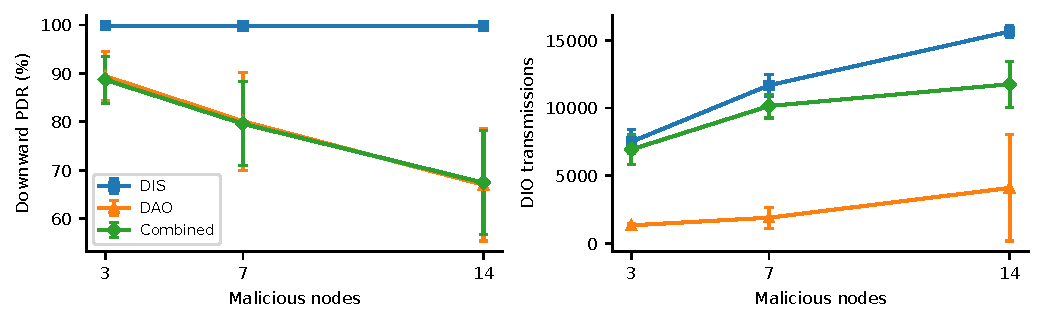
\includegraphics[width=.95\textwidth]{full_paper/generated/attack_damage.pdf}
\caption{Unprotected static-network impact of DIS, DAO, and combined attacks across attacker counts. Means and 95\% Student-$t$ intervals use ten seeds per condition. DIO totals follow the cumulative-counter reporting boundaries.}\label{fig:damage}
\end{figure*}

\subsection{Detection and Communication Service: RQ3}
\begin{table*}[t]
\caption{Original combined-attack comparison with seven malicious clients (seeds 1--10). Values are mean $\pm$ 95\% confidence-interval half-width, in percent. Detection is the historical network-level node-flag outcome; new post-onset events are evaluated separately.}\label{tab:mainresults}
\centering\footnotesize\begin{tabular}{@{}lrrrr@{}}
\toprule
Mobile (\%) & Method & Down PDR (\%) & TPR (\%) & FPR (\%) \\
\midrule
0 & RPL & 79.6$\pm$8.7 & -- & -- \\
0 & Secure-RPL & 77.4$\pm$12.1 & 97.1$\pm$6.5 & 0.0$\pm$0.0 \\
0 & DIS-FDM & 77.2$\pm$11.1 & 97.1$\pm$6.5 & 8.6$\pm$7.7 \\
0 & Li-MSD & 82.3$\pm$6.6 & 94.3$\pm$7.1 & 0.0$\pm$0.0 \\
0 & AEF fixed & 97.4$\pm$3.3 & 97.1$\pm$6.5 & 7.7$\pm$9.6 \\
0 & AEF learning & 98.3$\pm$1.6 & 97.1$\pm$6.5 & 16.8$\pm$15.4 \\
30 & RPL & 82.6$\pm$12.0 & -- & -- \\
30 & Secure-RPL & 80.8$\pm$11.1 & 100.0$\pm$0.0 & 0.0$\pm$0.0 \\
30 & DIS-FDM & 80.8$\pm$11.3 & 100.0$\pm$0.0 & 69.5$\pm$17.3 \\
30 & Li-MSD & 85.7$\pm$11.2 & 65.7$\pm$15.4 & 2.7$\pm$2.3 \\
30 & AEF fixed & 98.1$\pm$1.3 & 100.0$\pm$0.0 & 54.5$\pm$11.9 \\
30 & AEF learning & 96.4$\pm$3.8 & 100.0$\pm$0.0 & 55.0$\pm$12.6 \\
\bottomrule
\end{tabular}

\end{table*}

Table~\ref{tab:mainresults} and Fig.~\ref{fig:service} show the distinction between recognizing a malicious node and preserving routing service. With seven attackers in static networks, DIS-FDM and AEF learning have the same mean TPR, 97.14\%, while downward PDR is 77.19\% and 98.31\%, respectively. Secure-RPL has zero mean FPR in this cell but downward PDR of 77.40\%. Its DIS-specific response does not by itself correct the incorrect-parent DAO. AEF fixed also preserves substantial downward service (97.39\%). This pattern is consistent with a benefit from the DAO-aware handling shared by the AEF variants, not a detection-rate advantage attributable only to learning.

Mobility exposes a substantial cost. With seven attackers and 30\% mobility, AEF learning reaches mean downward PDR of 96.37\%, compared with 80.83\% for DIS-FDM, but its FPR is 55.00\%. AEF fixed has 98.10\% downward PDR and 54.55\% FPR. Li-MSD trades lower mean TPR (65.71\%) for a much lower FPR (2.73\%) and 85.71\% downward PDR. Thus, full AEF does not dominate the selected alternatives on all detection and service outcomes.

\begin{figure*}[t]
\centering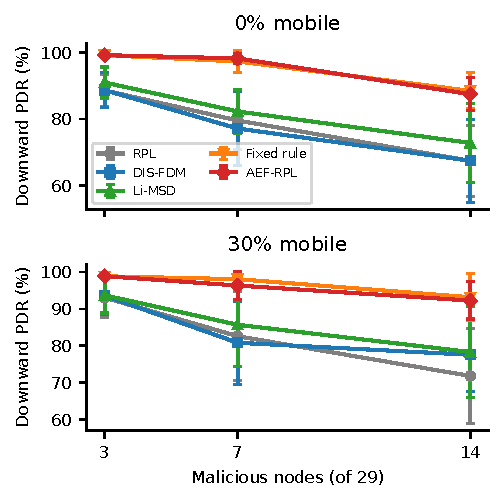
\includegraphics[width=.95\textwidth]{full_paper/generated/main_service.pdf}
\caption{Downward service under the combined attack in the original campaign. Increasing attacker count is crossed with static/mobile operation; error bars show 95\% intervals over ten seeds. High service does not imply low false isolation.}\label{fig:service}
\end{figure*}

The independent rate study uses seeds 21--30 and exact-matched benign references. At the default 3/2~s intervals, AEF learning achieves downward PDR of 95.73\% (static) and 98.04\% (mobile), compared with DIS-FDM's 78.70\% and 82.81\%. Table~\ref{tab:extension} reports macro-F1, ARI, and new-alert recall for the same cells. Li-MSD has higher macro-F1 than AEF in both conditions because its much smaller false-positive burden offsets missed attacker events. The mobile AEF FPR remains 45.00\%.

\begin{table}[t]
\caption{Default-rate extension (seven attackers, seeds 21--30): means on $[0,1]$, except ARI, which is a reference-normalized service ratio.}\label{tab:extension}
\centering\footnotesize\begin{tabular}{@{}lrrrr@{}}
\toprule
Mobile (\%) & Method & Macro-F1 & ARI & New recall \\
\midrule
0 & DIS-FDM & 0.939 & 0.741 & 0.986 \\
0 & Li-MSD & 0.974 & 0.791 & 0.943 \\
0 & AEF learning & 0.912 & 0.921 & 0.986 \\
30 & DIS-FDM & 0.641 & 0.800 & 1.000 \\
30 & Li-MSD & 0.925 & 0.847 & 0.800 \\
30 & AEF learning & 0.647 & 0.986 & 1.000 \\
\bottomrule
\end{tabular}

\end{table}
\begin{table}[t]
\caption{AEF-learning minus comparator downward-PDR differences in the same extension cells. Bootstrap intervals are unadjusted; $p_H$ uses the full rate-experiment Holm family.}\label{tab:effects}
\centering\footnotesize\begin{tabular}{@{}lrrrr@{}}
\toprule
Mobile (\%) & Comparator & $\Delta$ (pp) & 95\% paired CI & $p_H$ \\
\midrule
0 & DIS-FDM & 17.04 & [13.15, 21.17] & 0.172 \\
0 & Li-MSD & 11.09 & [7.54, 14.85] & 0.172 \\
30 & DIS-FDM & 15.23 & [7.24, 23.70] & 0.172 \\
30 & Li-MSD & 8.10 & [3.83, 13.06] & 0.172 \\
\bottomrule
\end{tabular}

\end{table}

Table~\ref{tab:effects} qualifies the evidence for the service differences. Against DIS-FDM, paired mean differences are +17.04 percentage points (static; bootstrap interval 13.15--21.17) and +15.23 points (mobile; 7.24--23.70). However, the broadly adjusted $p_H$ is .172 in both cells. We therefore report repeatable descriptive improvements and effect estimates without calling these extension comparisons statistically significant at the family-wise .05 level. The confidence interval and adjusted test answer different multiplicity questions.

\subsection{Timing, Missed Events, and Rate Robustness}
Fig.~\ref{fig:delay} shows new-alert delays with the fraction of events lacking a new post-onset flag. Pre-onset isolation is retained separately in the event table. Delays computed only for successful alerts cannot establish superiority when methods have different missed-event rates. In the mobile default-rate extension, mean per-run new-alert recall is 1.0 for DIS-FDM and AEF and .8 for Li-MSD. These observations concern one sustained event per attacker, not independent packet-level attacks or a family classifier.

Fig.~\ref{fig:rates} reports the joint rate perturbations. Longer intervals weaken the persistence signals used by the detectors. No interpolation to arbitrary attacker schedules is justified, and the coordinated interval changes do not establish which message type causes a performance change. The original window-sensitivity result and the added low-rate runs together argue for reporting the implemented temporal assumptions explicitly.

\begin{figure*}[t]
\centering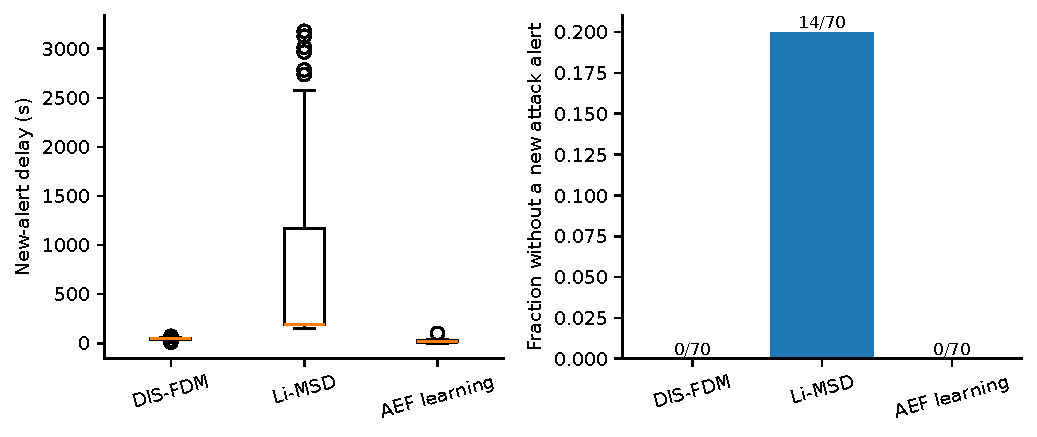
\includegraphics[width=.91\textwidth]{output/experiments/journal_extension/figures/detection_delay_and_missed_events.pdf}
\caption{New-alert timing in the mobile default-rate extension. The left panel conditions delay on successful new alerts; the right panel reports the number without such an alert. Existing pre-onset isolation is a separate logged state.}\label{fig:delay}
\end{figure*}
\begin{figure*}[t]
\centering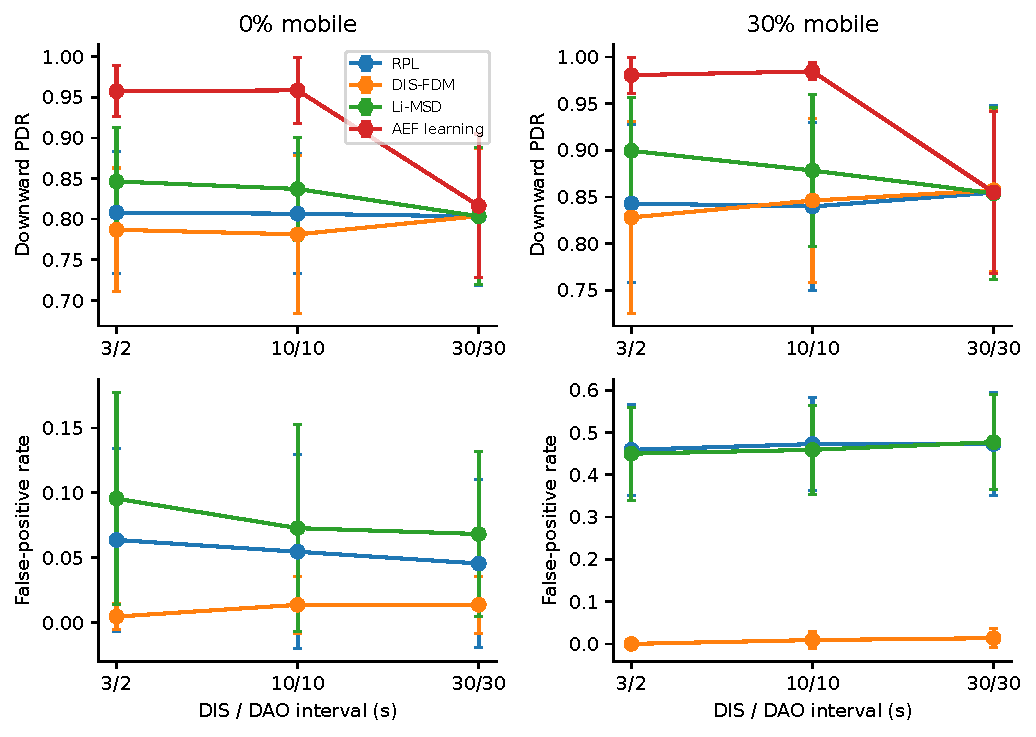
\includegraphics[width=.86\textwidth]{output/experiments/journal_extension/figures/rate_robustness.pdf}
\caption{Joint DIS/DAO rate robustness, ten seeds per cell. Top: downward PDR; bottom: FPR. Unprotected RPL has no detector FPR. Both attack intervals vary together.}\label{fig:rates}
\end{figure*}

\subsection{Learning and Architectural Contributions: RQ4}
The benign fresh-seed comparison does not support the proposed false-positive reduction. Across seeds 11--20, mobile FPR is 42.41\% with learning and 42.07\% with the fixed rule. The paired learning-minus-fixed mean difference is +0.345 percentage points (95\% paired-bootstrap interval 0.000--1.034; two-sided Wilcoxon $p=1.0$). This is a failure to demonstrate a benefit, not proof that the methods are equivalent. Mean blacklist operations are 1352.7 and 204.1 per run, respectively, showing that similar unique-node FPR can conceal substantial release/re-isolation churn.

The component study supplies a separate ten-seed assessment (Fig.~\ref{fig:ablation}). Under static combined attacks, full AEF has mean macro-F1 .901, whereas learning off has .971; their FPRs are 11.82\% and 3.18\%. Immediate DAO evidence has FPR 20.45\% and macro-F1 .833. Fixed calibration produces .918 macro-F1. In mobile conditions, full and learning-off macro-F1 both average .695, with FPR 38.18\%. None of these outcomes supports presenting learning as a consistently beneficial component.

Removing route repair reduces mean downward PDR from 97.61\% to 81.79\% (static) and 98.31\% to 81.52\% (mobile). Paired differences are +15.83 and +16.80 points, with bootstrap intervals 10.97--21.26 and 8.73--25.26, respectively. Both Holm-adjusted $p$ values are .176 under the full ablation family. This is descriptive evidence that the handling policy matters; broad inferential confirmation remains limited by sample size and multiplicity. Disabling only the DAO fusion mass causes a smaller service change, consistent with other DAO paths remaining active in that ablation.

\begin{figure*}[t]
\centering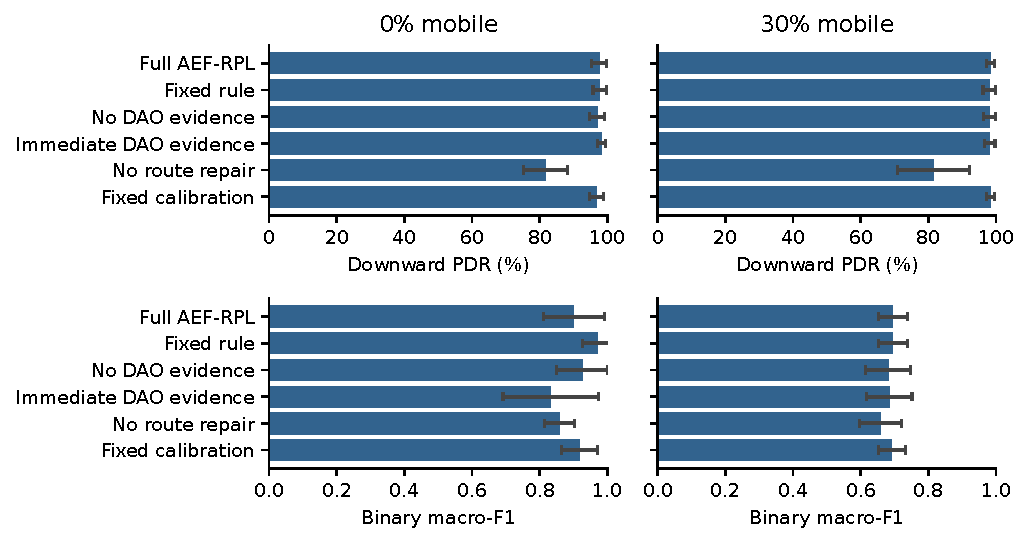
\includegraphics[width=.95\textwidth]{output/experiments/journal_extension/figures/component_ablation.pdf}
\caption{Component ablations under combined attacks, seeds 31--40. Bars show binary macro-F1 with 95\% intervals. The code label ``no dao evidence'' disables the fused DAO mass only; raw DAO observation, reward, and handling remain. ``No route repair'' retains the first-DAO forwarding allowance and other blacklist behavior.}\label{fig:ablation}
\end{figure*}

\subsection{Reception Loss and Operational Measurements: RQ5}
Fig.~\ref{fig:radio} crosses configured reception loss with mobility under combined attacks. These five-seed cells test measurement/communication degradation within the same radio model, not missing telemetry, sensor bias, or arbitrary physical faults. Downward PDR and false isolation must be considered together; a stable conditional delivery ratio does not show that all clients retain service. The corresponding run tables retain expected network-wide delivery and exact-reference ARI.

\begin{figure*}[t]
\centering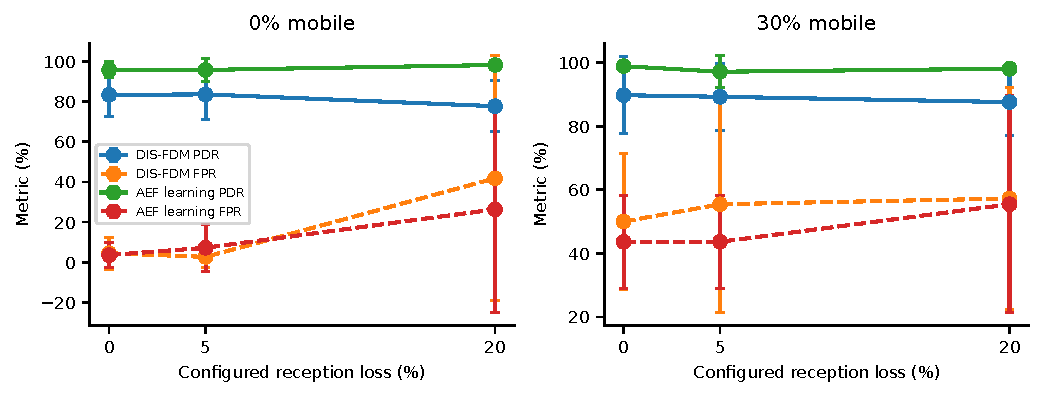
\includegraphics[width=.95\textwidth]{full_paper/generated/radio_loss.pdf}
\caption{Reception-loss sensitivity, five seeds per cell. Solid lines show downward PDR and dashed lines FPR. The x-axis is the complement of configured reception success, not the observed end-to-end packet-loss rate.}\label{fig:radio}
\end{figure*}

The host profiling measurements in Fig.~\ref{fig:cost} remain small relative to a 10~s decision window, but do not establish embedded real-time feasibility. In static attacked runs, the mean of run-median callback times is 2.57~$\mu$s for AEF and 2.02~$\mu$s for DIS-FDM; corresponding means of run 95th percentiles are 7.06 and 5.26~$\mu$s. In mobile attacked runs they are 5.15/10.28~$\mu$s for AEF and 3.51/7.06~$\mu$s for DIS-FDM. These are native host thread CPU measurements of the window callback, not detector-onset latency, complete pipeline cost, or constrained-mote speed. Simulation-derived power and native object-size outputs are available in the artifact with their measurement boundaries.

\begin{figure}[t]
\centering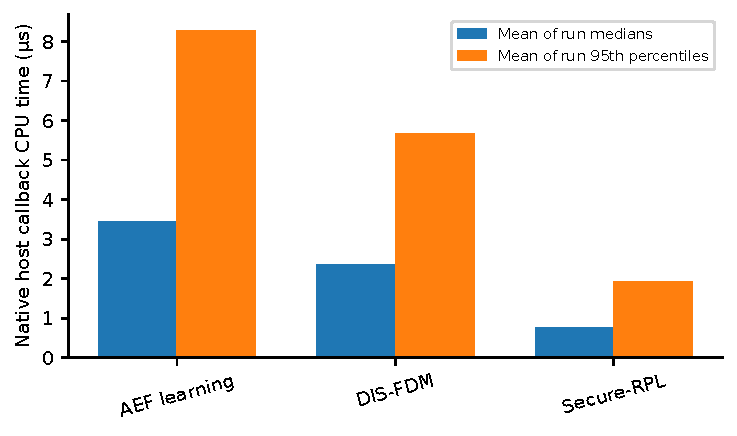
\includegraphics[width=\columnwidth]{output/experiments/journal_extension/figures/native_callback_cost.pdf}
\caption{Native host callback cost across the profiling cells. Bar values average run medians or run 95th percentiles; each method has 20 runs across workload/mobility cells. No target-MCU timing claim is made.}\label{fig:cost}
\end{figure}

\subsection{Large-Scale Feasibility and Failure Diagnosis}
All eight original attack-free scale diagnostics completed, but none passed the connectivity gate. At 500 nodes, 57.1--61.9\% of legitimate clients transmitted application traffic and expected upward delivery was 7.1--8.1\%. At 1000 nodes, participation was 29.3--32.9\% and expected upward delivery 1.6--3.6\%. Conditional downward PDR remained above 90\%; it therefore concealed poor network-wide participation. The simulated node positions are shown in Fig.~\ref{fig:layouts}; this figure depicts actual scenario coordinates, not verified usable routes.

An isolated eight-minute, 500-node trace with no attack and no defense retained stack warnings discarded by the usual application-only logger. It recorded 140 compressed-header/first-fragment fit rejections, 2126 CSMA neighbor-queue allocation drops, and 457 DAO-retry-exhaustion local repairs across 360 nodes. The pinned CSMA implementation defaults to two concurrent neighbor queues, separately from the increased packet-buffer pool. Long non-storing source routes can also exceed the first-fragment compressed-header capacity. These observations identify concrete drop mechanisms and the route-reset trigger, but do not assign every missed acknowledgment to one mechanism.

The corrective validation uses matched layouts to vary the CSMA neighbor-queue limit (16), extension-header compression (disabled while retaining IPv6 IPHC), and both changes. Twelve runs are planned across 500/1000 nodes and seeds 1--2. Their outcome and the subsequent 114-run attack matrix are not reported as completed here. Scalability remains an unresolved claim until corrective controls and the separately seeded defense comparisons finish.

\begin{figure*}[t]
\centering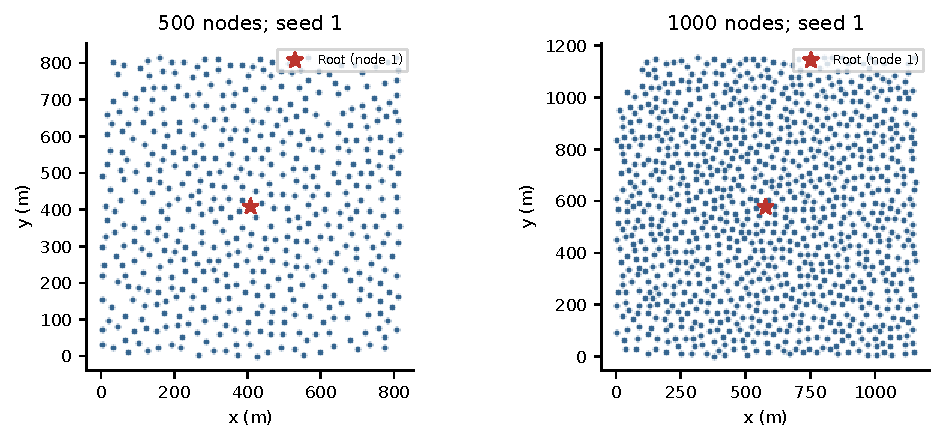
\includegraphics[width=.91\textwidth]{full_paper/generated/scale_layouts.pdf}
\caption{Actual seed-1 layouts for the 500- and 1000-node diagnostics; each dot is a simulated mote and the star is root node~1. Geometric connectivity does not establish RPL convergence or application reachability.}\label{fig:layouts}
\end{figure*}
